\documentclass[a4paper,11pt]{article}
\pdfoutput=1
\usepackage{jinstpub} % for details on the use of the package,                           please
                     % see the JINST-author-manual
\usepackage{xcolor,soul,framed} %,caption
\usepackage{mdwmath}
\usepackage{mdwtab}
\usepackage{eqparbox}
\usepackage{url}
\usepackage{dblfloatfix}    % To enable figures at the bottom of page
\usepackage{kantlipsum}     % for random text
\usepackage{hyperref}
\usepackage[export]{adjustbox}

\begin{document}
%\bstctlcite{IEEEexample:BSTcontrol}
    \title{Contaminate Imaging in Chicken Using CZT Detector}
    
\author[a,1]{Jericho~O'Connell,\note{Corresponding author.}}
\author[a]{Kevin J. Murphy}
\author[a]{Spencer M. Robinson}
\author[b]{Kris~Iniewski}% <-this % stops a space
\author[a]{Magdalena~Bazalova-Carter}

\emailAdd{jerichoo@uvic.ca}

\affiliation[a]{University of Victoria,\\3800 Finnerty Rd, Victoria, BC, Canada}
\affiliation[b]{Redlen Technologies,\\123 - 1763 Sean Heights
Saanichton, BC, Canada}

\abstract{
A 330 $\mu$m pitch  $8\times12$ Cadmium Zinc Telluride (CZT) detector with 6 energy bins is utilized to see potential benefits of its application in segmentation of soft tissue. Planar X-ray scans are completed using a table top set up consisting of a X-ray tube, and the CZT detector, both mounted on motion stages to allow for vertical and horizontal motion. A PMMA phantom with contaminates (glass, steel, plastic, polypropylene, and PFTE) was imaged as well as chicken flesh with contaminates (cartilage, bone, fat, plastic, wood, glass, rock, steel and aluminum) to determine there detectability given varying depths. These images were performed at 120 kVp, and 1 mA, with 1 second acquisition time. Given a Contrast to Noise Ratio (CNR) greater the 4 a computer is capable of accurately segmenting contaminates, this study looks to enquire about the potential of using Convolutional neural networks (CNN) to quickly sort flesh based on it components given the added detection ability capable with a multiple energy bin CZT detector.


% A rigorous method for automated soft tissue segmentation using planar kilovoltage (kV) imaging, a photon counting detector (PCD), and a convolutional neural network is presented. The goal of the project was to determine the optimum number of energy bins in a PCD for soft tissue segmentation. Planar kV X-ray images of solid water (SW) phantoms with varying depth of cartilage were generated with a cone-beam analytical method and parallel-beam Monte Carlo simulations. Simulations were preformed using 2 to 5 PCD energy bins with equal photon fluence distribution. Simulated image signal to noise ratio (SNR) was varied between 10 to 250 measured after transmission through 4 cm of SW. Algorithms using non-linear as well as linear regression were used to predict the amount of cartilage for every pixel of the phantom. These algorithms were evaluated based on the mean squared error (MSE) between their prediction and the ground truth. The best algorithm was used to decompose randomly generated SW and cartilage images with an SNR of 100. These randomly generated images trained a U-Net convolutional neural network to segment the cartilage in the image. The results indicated the smallest MSE occurred for non-linear regression with 4 energy bins over all SNR. The trained U-Net was able to correctly segment all regions of cartilage for the smallest amount of cartilage used (4 mm) and segmented the region with $>$ 99\% categorical accuracy by pixel. 
}

\maketitle
% * <jericho.oconnell@icr.ac.uk> 2018-08-29T22:15:14.220Z:
%
% ^.

\section{Introduction}

The modern workplace seeks efficiency through automation of human roles. When used properly, automation can increase production and lower cost. With automation, however, comes an increased pressure on quality control: Machines, unlike humans, traditionally lack the interpretive skill to asses their work. Current planar X-ray imaging capabilities are limited to the detection of large differences in material density. However, new solid state photon count detectors (PCDs) may allow for X-ray imaging to be extended to materials of similar composition. This application is particularly important to medical imaging where neighboring tissues often share similar composition. In this work, spectral imaging is examined for the detection of various contaminates in soft tissue. This is meant to be a direct application to planar medical imaging of soft tissues. However, these results apply equally to the planar X-ray discrimination of other materials with two components of similar composition. Other works have been done to investigate dual energy imaging in this application [1] [2], but the extension to more energies has not been seen.

This experiment looks to investigate the potential of planar imaging for the detection of contaminates in a PMMA phantom as well as chicken flesh. Contrast to Noise Ratio's (CNR's) will be examined for each energy bin to determine the effectiveness of having 6 separate energy bins for discernment between contrast agents. One aspect of this investigation is to examine the potential capabilities of spectral imaging in discerning between items of similar composition, such as cartilage, fat, and other tissues. An advantage of the Cadmium Zinc Telluride (CZT) crystal used is the potential to set multiple energy bins to detect for contaminates, this allows for each bin to be tailored to the potential contaminates imaged based on their respective K \& L edge values. 

With data collected we look to examine the ability of performing nondestructive testing (NDT) using spectral planar imaging, and determine how to accurately contaminate can be imaged while delivering a minimal radiation dose to the object imaged. This will refine our ability to detect different thickness of cartilage or fat in surrounding tissue while remain non-intrusive. In application the detection of these contaminates would be beneficial to the poultry industry in being able to determine the exact contents of poultry before being distributed and sold. 

Similar application can be seen in airport scanning devices where people can be scanned for various objects that are not allowed within airports in very short time frames with no damage to the body being scanned. For detection of contaminates within meats using an X-ray source the data acquisition and analysis must occur very quickly and use a low current X-ray source to remain cost effective. With the large increase in capabilities of machine learning methods such as CNN's, the potential to automate the detection of contaminates within meats using a pre-screening non intrusive testing method offers a large area for profitability. 

%Must add more paper that are being reference in this section: 	Papers about Airport Scanning, Jerichoos original simulations, Spectral Imaging of objects.




\section{Materials and Methods}
\label{sec:methods}

\subsection{Data Aquistion}
X-ray scans were performed on a PMMA phantom with 5 contaminates (steel, glass, plastic, polypropylene, and PFTE) as well as chicken flesh with various contaminates (bone, cartilage, fat, plastic, wood, glass, rock, steel, and aluminum).

Data was acquired using a CZT detector with a 8$\times$12 mm imaging array from Redlen Technologies. The 330 $\mu$m pitch high-flux CZT detector is 2mm thick and is able to operate at 250 $\frac{Mcps}{mm^2}$ without any signs of polarization. Travel Heat Method (THM) was adopted by Redlen Technologies when growing the CZT crystals used in the detector. These crystals were placed in a sensor that is connected to a photon counting ASIC which operates at rates of up to 62.5 $\frac{Mcps}{channel}$. This ASIC communicates with an external PC though LVDS I/Os via a programmable FPGA. The energies of photons incident with the detector are sorted into six energy bins by the ASIC. In the case of this experiment the energy bins were set to 16-33 keV, 33-41 keV, 41-50 keV, 50-90 keV, 90-120 keV, \& 120< keV.

The detector and X-ray source were both mounted on vertical and horizontal linear motion stages from Newport Corporations. These stages were oriented perpendicular to each other to allow for easy navigation while imaging the phantom, which was mounted between these two stages. The X-ray source used was a module XRS-160 from Comet Technologies. 

The PMMA phantom block as imaged in figure (1.C) was placed on the stage and the 3 smallest contaminates of each material were imaged. To image these contaminates each at different heights, the CZT detector and X-ray source were moved vertically in a uniform manner allowing for each material to be centered without any motion of the phantom block itself. Following the first round of data acquisitions a second block of 18mm PMMA was placed in front of the phantom block and images were acquired to determine the depth at which each contaminate could be visualized. 

In the case of the chicken flesh, each contaminate was able to fit in a phantom holder alongside the chicken. This block was placed on the stage and was able to be imaged in one scan per contaminate. 

Air scans were completed for each data acquisition and could then be processed using MATLAB (The Mathworks, Natick, MA) for image reconstruction and CNR calculations for each contaminate. During all scans the X-ray tube was using a cone beam operating at 1mA, 120 kV, with a 1mm focal spot. 

\begin{figure}[htbp]

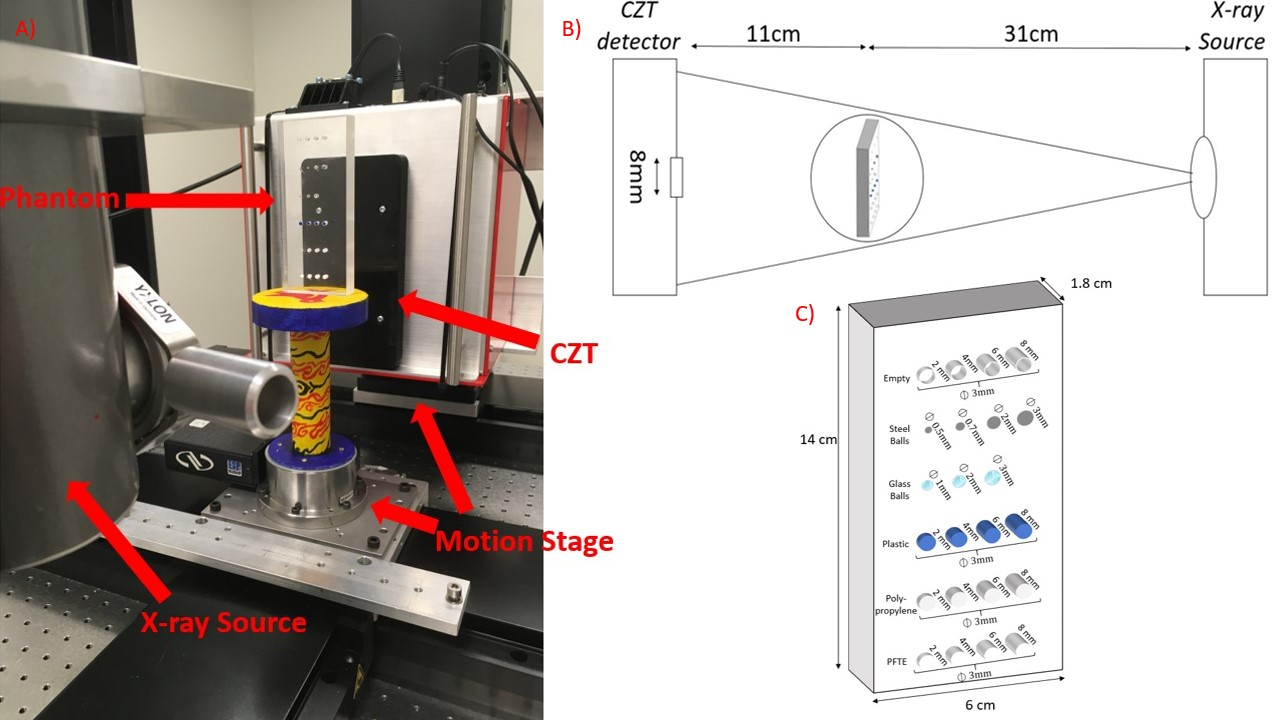
\includegraphics[width=\textwidth]{FullFigure.jpg}

\caption{A) Shows an image of the lab after data was acquired with different components as labeled. B) Is a schematic of the lab with distances from source to detector labeled. C) The layout for the phantom used with sizes of contaminates as labeled.}
\label{figcali}
\end{figure}

\subsection{Image Reconstruction}
\subsubsection{Spectral CT Image Reconstruction}
Python was used to collect and analyze data, while MATLAB was used for data processing and image reconstruction. The detector counts/intensity for an air scan ($I_0$) was used to normalize the counts/intensity with the phantom ($I$) and produce projections by the equation: 
\begin{equation}
    p = -\ln(I/I_0)
\end{equation}
These projections were then plotted to show the variance of attenuation through the phantom for each contaminate as imaged in Figure 2.A). 

\begin{figure}[htbp]
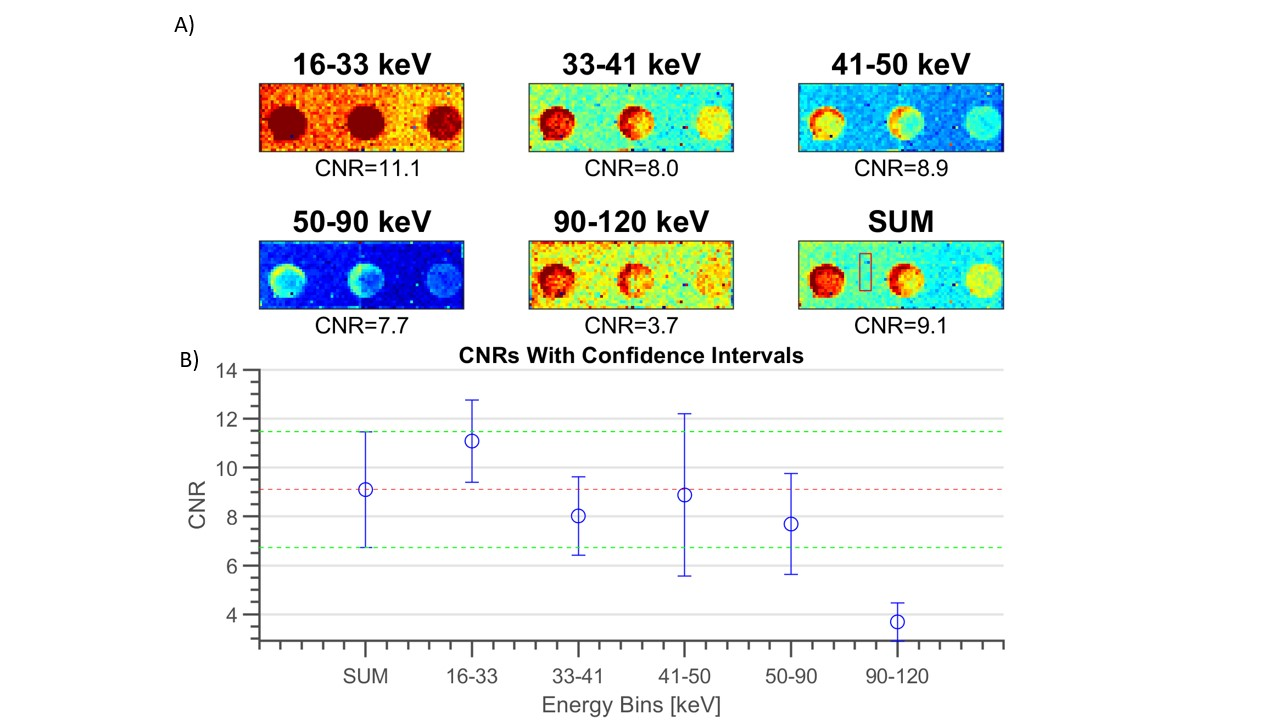
\includegraphics[width=\textwidth]{PTFE(Left).jpg}
\caption{A) CZT images for PFTE contaminate with CNR's calculated for each bin based on the ROI's as show in the SUM bin. B) CNR values for each bin with 99\% Confidence interval}
\label{figcali}
\end{figure}


\subsubsection{Contrast-to-Noise Ratio}
The Contrast to Noise Ratio (CNR) and a 99\% Confidence Interval was calculated for each energy bin based on ROI's selected by the user. The CNR's were calculated by taking the difference between the mean of each ROI $\mu_{\mathrm{background}}$ and $\mu_{\mathrm{phantom}}$ divided by the standard deviation in the phantom $\sigma_{\mathrm{phantom}}$, expressed by the equation: 

\begin{align}
    \mathrm{CNR} = \frac{\mu_{\mathrm{background}} - \mu_{\mathrm{phantom}}}{\sigma_{\mathrm{phantom}}} \\
\end{align}

A confidence interval was then produced using MATLAB's bootstrp function and is demonstrated in Figure 2.B). The selection of the ROI by the user allowed variance in  the CNR's when calculated, this is why a confidence interval was determine for each energy bin. 

\section{Results}
A CNR value of 4 or greater is necessary to effectively distinguish between a contaminate object and the surround background for a CNN. In the case of steel and glass it is evident that the CNR is much larger then 4 for nearly all images other then a 1mm diameter ball of glass within the 36mm of PMMA. The plastic/blue belt CNR was slightly above 4 for the 3rd and 4th energy bin in all images of then the 6mm long piece within the 36mm of PMMA. Polypropylene was effectively imaged with CNR's above 4 in at least 2 energy bins in all cases, CNR was largest in the 4th energy bin and was slightly less in the 3rd bin. PFTE images produced distinguishable CNR ratio's in half of the images taken, with the 6mm length being visible in both 18mm and 36mm of PMMA, and the 4mm being visible in 18mm but not 36mm, and not be distinguishable in either case for the 2mm length rod. The 1st energy bin (16-33 keV) had the largest CNR value in all but one case, but seems to be the best energy range to visualize PFTE in. 

\section{Discussion and Conclusions}

 \section*{Acknowledgments}

% or
\appendix{}
\section{Git Repository}




\bibliographystyle{JHEP}
\bibliography{references}


\vfill





%Removed by Kevin%
%This work aims to examine the potential of spectral imaging in nondestructive testing (DNT) what the minimal imaging parameters are for systems to be accurate. Specifically, to examine the detection of different thicknesses of cartilage under different xray exposures. To this aim, the independent variables in question will be signal to noise ratio (SNR) and thickness of cartilage in cm. The novelty of this work is twofold: The first novel component is a REDLEN cadmium zinc telluride semiconductor PCD. Secondly, the cartilage identification method is novel in that it extends dual energy extraction of Alvarez [3] to many energies. This method is coupled with a convolutional neural network (CNN) , the architecture being the U-Net achitecture which is shown to be optimal for segmentation [4]. And has also been used in k-edge imaging for spectral CT [5] Overall, this work aims to examine the application of CNNs and photon counting detectors (PCDs) in planar medical imaging.






% Can be used to pull up biographies so that the bottom of the last one
% is flush with the other column.
%\enlargethispage{-5in}



% that's all folks
\end{document}
% \title{Journal of Instrumentation (JINST) template}


% %% %simple case: 2 authors, same institution
% %% \author{A. Uthor}
% %% \author{and A. Nother Author}
% %% \affiliation{Institution,\\Address, Country}

% % more complex case: 4 authors, 3 institutions, 2 footnotes
% \author[a,b,1]{F. Irst,\note{Corresponding author.}}
% \author[c]{S. Econd,}
% \author[a,2]{T. Hird\note{Also at Some University.}}
% \author[c,2]{and Fourth}

% % The "\note" macro will give a warning: "Ignoring empty anchor..."
% % you can safely ignore it.

% \affiliation[a]{One University,\\some-street, Country}
% \affiliation[b]{Another University,\\different-address, Country}
% \affiliation[c]{A School for Advanced Studies,\\some-location, Country}

% % e-mail addresses: only for the corresponding author
% \emailAdd{first@one.univ}



% \abstract{Abstract...}



% \keywords{Only keywords from JINST's keywords list please}


% \arxivnumber{1234.56789} % only if you have one


% % \collaboration{\includegraphics[height=17mm]{example-image}\\[6pt]
% %   XXX collaboration}
% % or
% \collaboration[c]{on behalf of XXX collaboration}


% % if you write for a special issue this may be useful





% \begin{document}
% \maketitle
% \flushbottom

% \section{Introduction}
% \label{sec:intro}

% The modern production line seeks efficiency through automation of human roles. When used properly, automation can increase production and lower cost. With automation, however, comes an increased pressure on quality control: Machines, unlike humans, are not expected to know if the product is contaminated by their actions. The ideal quality control in these situations is what is known as nondestructive testing (NDT), testing that leaves the product unchanged. The ideal NDT method is the use of XRay imaging. Current XRay imaging capabilities are limited to the detection of large differences in material density. However, new photon count detectors (PCDs) allow for XRay imaging to be extended to materials of similar composition. This application is particularly important in the meat processing industry where cartilage and tissue share similar compositions.

% In this work, spectral imaging is examined for the detection of cartilage in soft tissue. This is meant to be a direct application to the poultry industry. However, these results apply equally to the planar XRay discrimination of other materials with two components of similar composition. Other works have been done to investigate dual energy imaging in this application (???), but the extension to more energies has not been seen.

% It is important to note some other considerations in this problem: Firstly, this system must image objects on a conveyor belt moving at 0.5 m/s. And secondly to be cost effective the xray tube should be one with low current. Thus when discussing this problem it is essential to look at xray imaging for a photon starved system. 

% This work aims to examine exactly what the minimal imaging parameters are for systems to be accurate. Specifically, to examine the detection of different thicknesses of contaminant under different xray exposures. To this aim, the independent variables in question will be signal to noise ratio (SNR) and thickness of cartilage in cm.

% The novelty of this work is twofold: The first novel component is the modeling of a REDLEN cadmium zinc telluride semiconductor PCD. Secondly, the cartilage identification method is novel in that it extends dual energy extraction of (???) to many energies. This method is coupled with a convolutional neural network (CNN) , the architecture being the U-Net achitecture which is shown to be optimal for segmentation. Overall, this work aims to examine the application of CNNs and photon counting detectors (PCDs) in nondestructive imaging.

% \section{Methods}
% \label{sec:methods}

% An overview of the total work flow can be seen in figure~\ref{fig:i}:


% \begin{figure}[htbp]
% \centering % \begin{center}/\end{center} takes some additional vertical space
% \includegraphics[width=\textwidth]{figures/Slide4.jpg}
% \qquad
% % "\includegraphics" from the "graphicx" permits to crop (trim+clip)
% % and rotate (angle) and image (and much more)
% \caption{\label{fig:i} Complete work flow U-Net image reproduced with permission (???) from ....}
% \end{figure}

% Steps 1 (Image Simulation) and 2 (Multi-Energy Subtraction) are used to optimize the imaging parameters while the third step (Image Segmentation and Classification) is used to determine the limitations of the higher level classification.

% \subsection{Image Simulation}
% \subsubsection{Phantoms, Spectra and General Parameters}

% The phantoms used in this study were composed of Cartilage and Solid Water, the exact composition of the cartilage follows the ICRU-44 guidelines and the water is that of Watanabe 1999. 

% Table(*???)

% Three seperate phantoms were modeled of three diferent water thickness 8,  6, and 4 cm respectively. These thicknesses were chosen to span the range of thicknesses expected in the calibration, smaller phantoms were investigated but resulted in less failure of differentiation. In this phantom smaller inserts of 0:4 cm in 0.5cm increments were embedded, it is noted that the best interpolation would be the use of the Chebyshev nodes for this range as proposed by (???) however it has also been demonstrated that machinists prefer lengths that are rational numbers.

% \begin{figure}[htbp]
% \centering % \begin{center}/\end{center} takes some additional vertical space
% 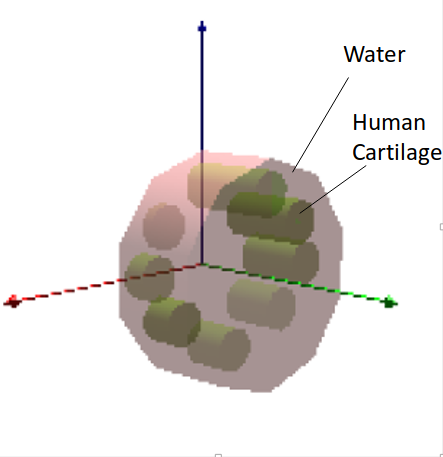
\includegraphics[width=0.4\textwidth]{figures/phantom.png}
% \qquad
% 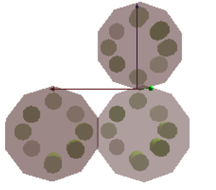
\includegraphics[width=.4\textwidth,]{figures/phantom3.png}
% % "\includegraphics" from the "graphicx" permits to crop (trim+clip)
% % and rotate (angle) and image (and much more)
% % "\includegraphics" from the "graphicx" permits to crop (trim+clip)
% % and rotate (angle) and image (and much more)
% \caption{\label{fig:i}  An image of one of the phantoms and all three}
% \end{figure}

% A similar phantom was used for the validation step save but with inserts of 0.4:3.9 cm in 0.5 cm increments.

% The spectra used was a simple 60 kVp spectrum with generated from a tungsten anode with 0.8 mm beryllium, 30 cm air and 0.1 mm copper filtration. The detector was an ideal integrating detector over the energy range indicated 

% A note should be made on the binning of the energies, energy bins for all of the simulation were calculated so as to have equal fluency in the each energy bin. These bins were calculated by integrating over the desired fraction of the spectra. This was done for optimal statistics as noise increases quadratically with decreasing signal equal fluence results in the best average signal to noise in the images. 

% \subsubsection{Analytical}

% Two separate types of simulations were preformed in this work, the first image simulation method uses Imasim (???) a ray tracing application that provides perfect ray tracings, Gaussian random noise was added to the images to mimic the Poisson statistics that occur in a normal image, the imaging parameters were made to the specifications of the REDLEN detector :

% table()

% \subsubsection{Monte Carlo}

% A monte carlo simulation was done using Geant4 extended by TOPAS, the spectrum was sampled from a analytically simulating with 89 points sampled over the spectra. For each phantom thickness 10 trials were preformed with different random number seeds with 5000000 photons each, these trails were summed to make up the images with the different signals. Complete imaging parameter files can be found in the github repository.


% \subsection{Multi-Energy Subtraction}


% Alvarez et al. mention many times in various papers that there is no improvement to dual energy subtraction when using more energies. This stems from the fact that the photoelectric component and the compton scattering component of the photon interactions fully describe the system, therefore two components can span this space and further images will just give linearly dependant information. In less words;



% \begin{equation}
% \label{eq:1}
% \mu(x,y,E) = a_1(x,y) \frac{1}{E^3}+a_2(x,y) f_{KN}(E)
% \end{equation}

% Where x, y and E need no explanation $\mu$ is the attenuation and $a_1, a_2 $ are coefficients for the photoelectric effect and Compton scattering component and $f_{KN}(E)$ is the Klein-Nishina function.

% However the finding of these coefficients is generally left to a least squares fitting of the material thicknesses $A_1, A_2$ to the log intensity $I_{energy 1}, I_{energy 2}$ of the image to find the parameters ${k_n}, {l_n}$ (ref ref ref???)


% \begin{subequations}\label{eq:t}
% \begin{align}
% \label{eq:t:1}
%  \ln(I_{energy 1}) = k_1 A_1 + k_2 A_2 +k_3A_1^2 +k_4 A_2^2 +k_5 A_1A_2 
% \\
% \label{eq:t:2}
% \ln(I_{energy 2}) = l_1 A_1 + l_2 A_2 +l_3A_1^2 +l_4 A_2^2 +l_5 A_1A_2 
% \end{align}
% \end{subequations}

% However this practise is not likely to produce the intended parametrization of the intensity of the image as a function of the Compton scattering and Photoelectric effect, instead is mush more likely to fit to the pixel intensity. To give an example, a least squares fit of thickness of bone $(A_1)$ and brain $(A_2)$ to one image will generate fit coefficients that map pixel intensity to bone thickness, since one cannot parametrize decompose an image into compton scattering and photoelectric effect in one image. This demonstrates that there is other information for the least squares fit to calibrate on. Given this it is safe to assume that when given more images the coefficients still have the possibility of fitting based off of the intensity rather than the CS/PE. Since the fit is not based entirely off of CS/PE it is possible that more images will give a better fit that will be based more on the CS/PE components in the material and less on the raw pixel intensity.

% Thus the idea of more energies being unececessary was put on hold and \ref{eq:y} was bravely extended to n energies as

% \begin{subequations}\label{eq:p}
% \begin{align}
% \label{eq:p:1}
% A_1 = \sum_{m=1}^n k_{m} \ln(I_{m})  +\sum_{j=1}^n  k'_{j,m} \ln(I_{j}) \ln(I_{m})
% \\
% \label{eq:p:2}
% A_2 = \sum_{m=1}^n l_{m} \ln(I_{m})  +\sum_{j=1}^n  l'_{j,m} \ln(I_{j}) \ln(I_{m})
% \end{align}
% \end{subequations}


% \subsubsection{Least-Squares Fitting}

% The least squares regression used was similar to what is described in \ref{eq:p} extended to n energies
% the intensities used in the fit were taken from the circular inserts of the phantom.

% \subsubsection{Non-Linear Fitting}

% The same equation \ref{eq:p} was fit using a feed forward neural network (MATLAB feedforwardnet(???)), the hyper parameters used were the defaults save the number of hidden layers was optimized individually for each combination of SNR by running 10 trials each for 5 to 100 layers in 5 layer interval, the optimal amount of layers was then selected as the result with the lowest mean squared error MSE on the validation data.

% \subsection{Image Segmentation and Classification}

% The input for the CNN is generated randomly assigned polygons as the background, these polygons are assigned image values taken from the validation images in Imasim with Poisson noise added to get the desired signal to noise ratio. The background polygons are composed of water in this way. The foreground is composed of circular regions of differing thicknesses of combined water and cartilage again taken from the Imasim validation data set, the U-Net is also provided a segmentation for training as seen in figure \ref{fig:j}. The exact hyperparameters for the network can be found at github (???).


% \begin{figure}[htbp]
% \centering % \begin{center}/\end{center} takes some additional vertical space
% 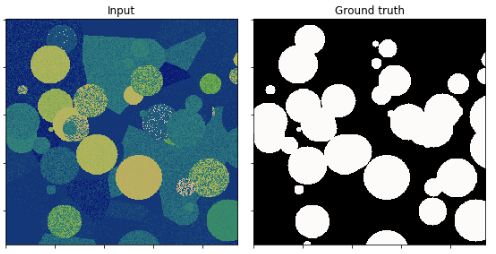
\includegraphics[width=\textwidth]{figures/CNN_val.png}
% \qquad
% % "\includegraphics" from the "graphicx" permits to crop (trim+clip)
% % and rotate (angle) and image (and much more)
% \caption{\label{fig:j} Complete work flow U-Net image reproduced with permission (???) from ....}
% \end{figure}

% \section{Results}

% The linear and non-linear regression were evaluated by means of CNR, MSE as a function of amount cartilage ($T_c$) and SNR. With the CNR and SNR defined relative to 4cm of water, specifically

% \begin{equation}
% \label{eq:f}
% CNR = \frac{|I^m_{ROI} - I^m_{H_2O}|}{\sqrt{\sigma^2_{ROI} + \sigma^2_{H_2O}}}
% \end{equation}
% The CNR was bootstrapped to the 95\% confidence interval which is shown as a band in figure \ref{}

% If you want some equations without the tag (number), please use the available
% starred-environments. For example:
% \begin{equation*}
% x = 1
% \end{equation*}

% The amsmath package has many features. For example, you can use use
% \texttt{subequations} environment:
% \begin{subequations}\label{eq:y}
% \begin{align}
% \label{eq:y:1}
% a & = 1 
% \\
% \label{eq:y:2}
% b & = 2
% \end{align}
% and it will continue to operate across the text also.
% \begin{equation}
% \label{eq:y:3}
% c = 3
% \end{equation}
% \end{subequations}
% The references will work as you'd expect: \eqref{eq:y:1},
% \eqref{eq:y:2} and \eqref{eq:y:3} are all part of \eqref{eq:y}.

% A similar solution is available for figures via the \texttt{subfigure}
% package (not loaded by default and not shown here).
% All figures and tables should be referenced in the text and should be
% placed on the page where they are first cited or in
% subsequent pages. Positioning them in the source file
% after the paragraph where you first reference them usually yield good
% results. See figure~\ref{fig:i} and table~\ref{tab:i}.

% \begin{figure}[htbp]
% \centering % \begin{center}/\end{center} takes some additional vertical space
% \includegraphics[width=.4\textwidth,trim=30 110 0 0,clip]{example-image-a}
% \qquad
% \includegraphics[width=.4\textwidth,origin=c,angle=180]{example-image-b}
% % "\includegraphics" from the "graphicx" permits to crop (trim+clip)
% % and rotate (angle) and image (and much more)
% \caption{\label{fig:i} Always give a caption.}
% \end{figure}


% \begin{table}[htbp]
% \centering
% \caption{\label{tab:i} We prefer to have borders around the tables.}
% \smallskip
% \begin{tabular}{|lr|c|}
% \hline
% x&y&x and y\\
% \hline
% a & b & a and b\\
% 1 & 2 & 1 and 2\\
% $\alpha$ & $\beta$ & $\alpha$ and $\beta$\\
% \hline
% \end{tabular}
% \end{table}

% We discourage the use of inline figures (wrapfigure), as they may be
% difficult to position if the page layout changes.

% We suggest not to abbreviate: ``section'', ``appendix'', ``figure''
% and ``table'', but ``eq.'' and ``ref.'' are welcome. Also, please do
% not use \texttt{\textbackslash emph} or \texttt{\textbackslash it} for
% latin abbreviaitons: i.e., et al., e.g., vs., etc.



% \section{Sections}
% \subsection{And subsequent}
% \subsubsection{Sub-sections}
% \paragraph{Up to paragraphs.} We find that having more levels usually
% reduces the clarity of the article. Also, we strongly discourage the
% use of non-numbered sections (e.g.~\texttt{\textbackslash
%   subsubsection*}).  Please also see the use of
% ``\texttt{\textbackslash texorpdfstring\{\}\{\}}'' to avoid warnings
% from the hyperref package when you have math in the section titles



% \appendix
% \section{Some title}
% Please always give a title also for appendices.





% \acknowledgments

% This is the most common positions for acknowledgments. A macro is
% available to maintain the same layout and spelling of the heading.

% \paragraph{Note added.} This is also a good position for notes added
% after the paper has been written.





% % We suggest to always provide author, title and journal data:
% % in short all the informations that clearly identify a document.

% \begin{thebibliography}{99}

% \bibitem{a}
% Author, \emph{Title}, \emph{J. Abbrev.} {\bf vol} (year) pg.

% \bibitem{b}
% Author, \emph{Title},
% arxiv:1234.5678.

% \bibitem{c}
% Author, \emph{Title},
% Publisher (year).


% % Please avoid comments such as "For a review'', "For some examples",
% % "and references therein" or move them in the text. In general,
% % please leave only references in the bibliography and move all
% % accessory text in footnotes.

% % Also, please have only one work for each \bibitem.


% \end{thebibliography}
% \end{document}
